\documentclass[tikz,border=0pt]{standalone}
\usepackage{pgfplots}
\usepackage{xcolor}
\usetikzlibrary{arrows}
\usetikzlibrary{arrows.meta}

% original colors
\definecolor{color1}{RGB}{166,118,29}
\definecolor{color2}{RGB}{217,95,2}
\definecolor{color3}{RGB}{231,41,138}
\definecolor{color4}{RGB}{117,112,179}
\definecolor{color5}{RGB}{27,158,119}
\definecolor{color6}{RGB}{102,166,30}
\definecolor{color7}{RGB}{230,171,2}

\begin{document}
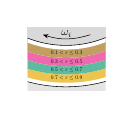
\begin{tikzpicture}
    \clip (-0.487, -1.100) rectangle (0.502, -1.9);

    % Outer cylinder and water inside
    \fill[fill=gray!20] (0, 0) circle (2.200);
    \draw[color=black, fill=white, very thin] (0, 0) circle (1.851);

    %0.7 < r < 0.9
    \fill[color=black, very thin, fill=color7!70] (0, 0) circle (1.799);
    \fill[color=black, very thin, fill=white] (0, 0) circle (1.693);
    \node[align=center] at (0.0075,-1.746) {\scalebox{0.2}{$0.7 < r \leq 0.9$}};

     %0.5 < r < 0.7
    \fill[color=black, very thin, fill=color5!70] (0, 0) circle (1.693);
    \fill[color=black, very thin, fill=white] (0, 0) circle (1.588);
    \node[align=center] at (0.0075,-1.641) {\scalebox{0.2}{$0.5 < r \leq 0.7$}};

    % 0.3 < r < 0.5
    \fill[color=black, very thin, fill=color3!70] (0, 0) circle (1.588);
    \fill[color=black, very thin, fill=white] (0, 0) circle (1.483);
    \node[align=center] at (0.0075,-1.536) {\scalebox{0.2}{$0.3 < r \leq 0.5$}};

    % 0.1 < r < 0.3
    \fill[color=black, very thin, fill=color1!70] (0, 0) circle (1.483);
    \fill[color=black, very thin, fill=white] (0, 0) circle (1.378);
    \node[align=center] at (0.0075,-1.425) {\scalebox{0.2}{$0.1 < r \leq 0.3$}};

    % inner cylinder
    \draw[color=black, fill=gray!30, very thin] (0, 0) circle (1.325);

    \coordinate (a) at (0.307, -1.190);
    \coordinate (b) at (-0.293, -1.190);
    \draw[black, very thin, -{Stealth[scale=0.5]}]
    (a) to [out=197, in=343] node[above=-3] {\scalebox{0.4}{$\omega_i$}} (b);
    %\path[-{Stealth[scale=0.5]}] (a) edge[bend left] (b);

\end{tikzpicture} 
\end{document}
